\section{Reasoning}
\label{sec-reasoning}

According to our observation,  an {\em incomplete} \kw{EAG} isn't well satisfying of answering the question because of the insufficient attributes.
To infer the hidden attributes, 
%In our proposed method, 
an inference graph is constructed accordingly.  
we briefly introduce the construction below. 

\subsection{Construction of Inference Graph}
To take advantage of the prior information and increase the generalization ability of the proposed model, our inference graph is constructed using Bayesian network.
Mathematically, Bayesian network \cite{friedman1997bayesian} can be described by a pair $\mathfrak{B}=<\mathcal{G},\varTheta_\mathcal{G}>$. 
Here, the notation $\mathcal{G}$ is a directed acyclic graph, of which the $i$-th vertex corresponds to a random variable $X_i$, and the edge between two connected vertexes indicates the dependency. 
Additionally, the second item $\varTheta_\mathcal{G}$ is a set of parameters used to quantify the dependencies in $\mathcal{G}$.
Denoted by $\text{Pa}(X_i)$ the attributes of the parents of $X_i$, 
the parameter of $X_i$ is represented by  $\theta_{X_i | \text{Pa}(X_i)} = P_\mathfrak{B}(X_i| \text{Pa}{(X_i)})$.
%We use the notation $\theta_{X_i | \text{Pa}(X_i)} = P_\mathfrak{B}(X_i| \text{Pa}{(X_i)})$ to denote the parameter of $X_i$, of which $\text{Pa}(X_i)$ is the attributes of the parents of $X_i$.
With the notations above, the joint probability distribution of Bayesian network is given by:

\begin{equation}\label{eq:BNOri}
\small
P_\mathfrak{B}(X_1, \cdots, X_n) = 
\prod_{i=1}^{n} P_\mathfrak{B}(X_i| \text{Pa}{(X_i)})=
\prod_{i=1}^{n} \theta_{X_i | \text{Pa}(X_i)}
%\theta_{x_1|\text{Pa}_1(\mathbf{x})}\theta_{x_2|\text{Pa}_2(\mathbf{x})}\cdots \theta_{x_n|\text{Pa}_n(\mathbf{x})}
\end{equation}
\vspace{-1ex}

In our inference graph, the role of Bayesian network is to predict the object class when given the attributes $\{X_i\}_{i=1}^n$ as input. In the sense of probability, the object class is also a variable \cite{koller2009probabilistic}.
Defined by $X_0=Y$ the class variable, the network now has one extra vertex $X_0$.
In order to infer the class attribute, and according to the Bayesian rule, our problem becomes:

\vspace{-1ex}
\begin{align}\label{eq:BNWithCls}
\begin{split}
P_\mathfrak{B}(Y|{X}) & = 
\frac{ P_\mathfrak{B}(Y) P_\mathfrak{B}({X}|Y) }{P_\mathfrak{B}({X})}\\
&=\frac{ \theta_{Y|\text{Pa}({X}_0)} \prod_{i=1}^{n} \theta_{X_i|Y, \text{Pa}({X}_i)} }{ \sum_{y'\in \mathcal{Y}} \theta_{y'|\text{Pa}({X}_0)} \prod_{i=1}^{n} \theta_{X_i|y', \text{Pa}({X}_i)} }
\end{split}
\end{align}
where $\mathcal{Y}$ is the set of classes.

\begin{figure}[tb]
\centering
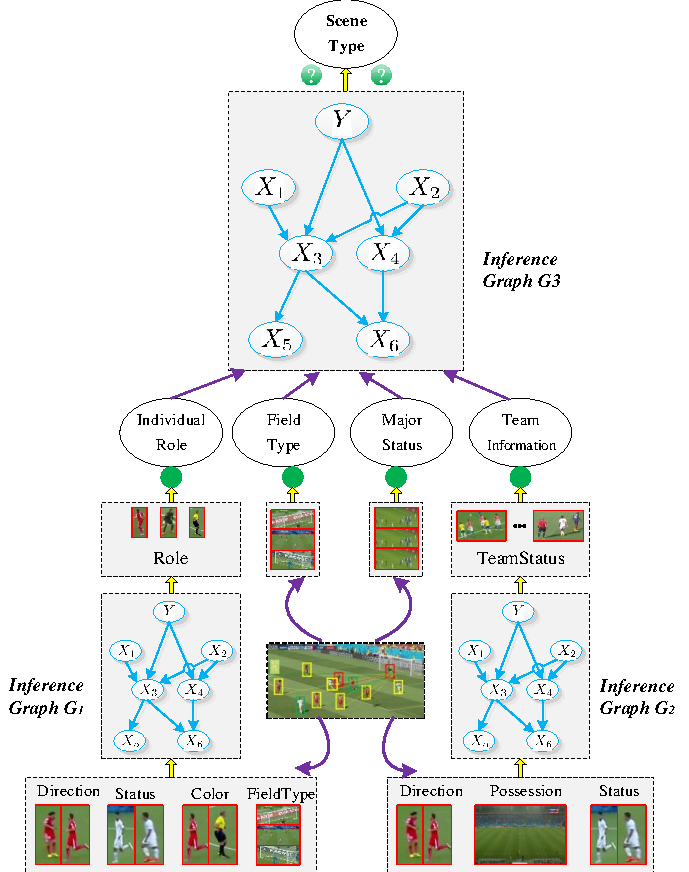
\includegraphics[width=\columnwidth]{inferGraph}
\caption{Schematic diagram of inference graph.}
\vspace{-4ex}
\label{fig:inferGraphWork}
\end{figure}

\subsection{Learning the Structure of Inference Graph}

In the context of Na\"{i}ve Bayes, 
the structure of $P_\mathfrak{B}(Y|{X})$ is simplified by taking the class variable as the root, and all attributes are conditionally independent when taking the class as a condition \cite{petitjean2018accurate}. As a consequence, the attribute class can be explicitly inferred by:

\begin{equation}\label{eq:BN-naiveBayes}
P_\mathfrak{B}(Y| {X}) = c \cdot \theta_Y \prod_{i=1}^{n}\theta_{X_i|Y}
\end{equation}
where $c$ is a scale factor that makes the calculation being a distribution: $c=\sum_{y'\in \mathcal{Y}}  \theta_{y'} \prod_{i=1}^{n}\theta_{X_i|y'}$.

One can observe from Eq.\eqref{eq:BN-naiveBayes} that Na\"{i}ve Bayes simplifies the complexity of Bayesian network. As can be validated by the experimental results, the simple model works excellently to our problem. 

\autoref{fig:inferGraphWork} summarizes the processes of our inference graph, where three graphs are constructed according to the tasks involved. First, the role of a candidate is inferred from $G_1$, in which four different kinds of features are extracted from the scene image. Then, the team status is inferred through the second inference graph $G_2$, but with different features as input. Next, we use the inferred information, along with the other information can be directly detected from the scene image, to infer the information of the whole scene.
The scene information is then fed into the incomplete \kw{EAG} so that a complete \kw{EAG} can be obtained. 

%\begin{figure}[tb!]
%\centering
%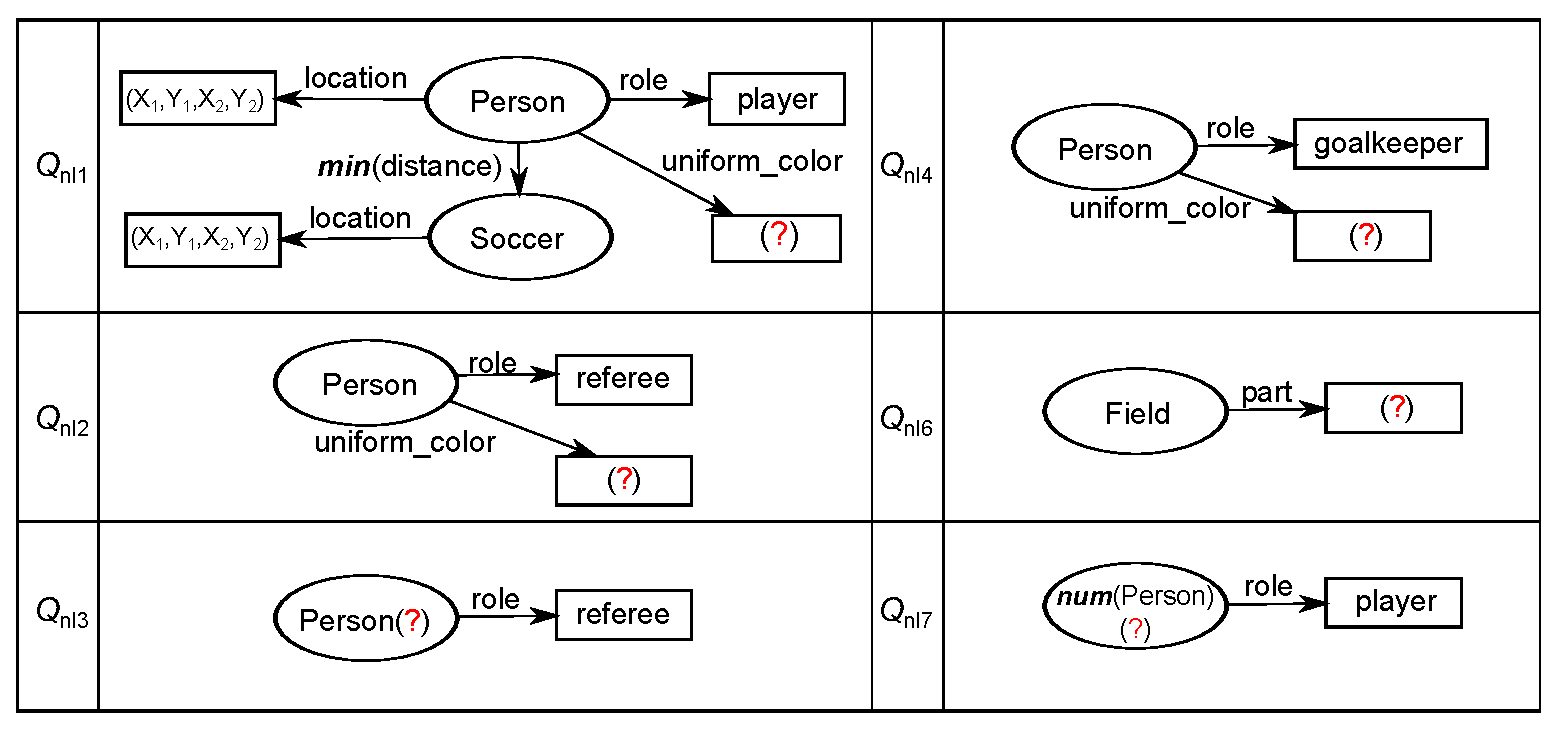
\includegraphics[width=\columnwidth]{queries.eps}
%\caption{Query graphs}
%\label{fig:queries}
%\end{figure}